\section{Version control using Helix Core\textsuperscript{\texttrademark}}
In this section, a very basic 2D game is created with the game engine Godot. The development process is version 
controlled using the Helix Core application to demonstrate the major steps and show the differences compared to 
traditional SW development workflow.
\begin{itemize}
    \item centralized version control system: files are maintained on centralized server
    \item files are stored in depots: typically 1 depot per project
    \item workspace: mapping of relevant files between local machine and server
\end{itemize}

\subsection{Setup Helix Core}
The setup of Helix Core follows the instructions from the 
\href{https://help.perforce.com/helix-core/quickstart/Content/quickstart/admin-install-linux.html}{\color{blue}{Helix Core Server Administrator Guide}}
relevant for Linux (Ubuntu) systems. The following commands were issued for setting up the version control application, as 
can be found in the aformentioned documentation.
\begin{enumerate}
    \item Download perforce public key
    \begin{verbatim}
        $ wget https://package.perforce.com/perforce.pubkey
    \end{verbatim}
    \item Obtain the fingerprint of the public key and verify
    \begin{verbatim}
        $ gpg -n --import --import-options import-show perforce.pubkey
        $ gpg -n --import --import-options import-show perforce.pubkey | 
        grep -q "E58131C0AEA7B082C6DC4C937123CB760FF18869" && echo "true"
    \end{verbatim}
    \item Add the public key to your keyring
    \begin{verbatim}
        $ wget -qO - https://package.perforce.com/perforce.pubkey | 
        sudo apt-key add -
    \end{verbatim}
    \item Create a new file for the Perforce repository
    \begin{verbatim}
        $ sudo nano /etc/apt/sources.list.d/perforce.list
    \end{verbatim}
    \item In the new file, input the following line
    \begin{verbatim}
        deb http://package.perforce.com/apt/ubuntu focal release
    \end{verbatim}
    Make sure the version matches the Linux/Ubuntu version of the machine's system. E.g 'focal' needs to be replaced by
    'jammy' if the most recent Linux/Ubuntu LTS version is running on the machine.
    \item Update machine and install Helix Core
    \begin{verbatim}
        $ sudo apt-get update
        $ sudo apt-get install helix-p4d
    \end{verbatim}
    \item Run configure file
    \begin{verbatim}
        $ sudo /opt/perforce/sbin/configure-helix-p4d.sh
    \end{verbatim}
    During the installation process, I had problems with this step when I tried to remove and install the helix-p4d
    package. The correct way of removing all related data is summarised as follows:
    \begin{itemize}
        \item Remove package
        \begin{verbatim}
            $ sudo apt-get remove helix-p4dctl
            $ sudo apt-get purge helix-p4dctl
        \end{verbatim}
        \item For some reasons, the file \colorbox{blue!30}{/etc/perforce/p4dctl.conf.d/p4d.template} was missing after
        these steps. The file was recreated with below content (downloaded from \href{https://portal.perforce.com/s/article/15056}{\color{blue}{here}} 
        and slightly modified) and the install process worked again.
        \begin{verbatim}
            p4d %NAME%
            {
                Owner    =    perforce
                Execute  =    /opt/perforce/sbin/p4d
                Umask    =    077

                # Enabled by default.
                Enabled  =    true

                Environment
                {
                    P4ROOT    =    %ROOT%
                    P4SSLDIR  =    ssl
                    PATH      =    /bin:/usr/bin:/usr/local/bin:...
                    /opt/perforce/bin:/opt/perforce/sbin

                # Enables nightly checkpoint routine
                # This should *not* be considered a complete backup...
                solution
                MAINTENANCE =     true
                }
            }
        \end{verbatim}
    \end{itemize}
    \item Download visual interface (p4v) from 
    \href{https://www.perforce.com/downloads/helix-visual-client-p4v}{\color{blue} Download Page}.
    P4v is the client application commnicating with the server. Server in this case is created on local machine. In case of
    reinstall, the P4V client might also need to be unpacked again so that the already created workspaces do not block
    the execution.
    \item Additional config steps
    \begin{verbatim}
        $ export P4PORT=ssl:1666
        $ export P4USER=super
        # add the following line to ~/.bashrc
        export PATH=${PATH}:~/perforce/p4v-2023.3.2495381/bin
    \end{verbatim}
    \item Login and start p4v
    \begin{verbatim}
        $ p4 login
        $ p4v # launches GUI
    \end{verbatim}
\end{enumerate}
Having done the above steps, the GUI can be launched bringing up the screen below. The location of the server (where
all shared files/projects are stored) \colorbox{blue!30}{/opt/perforce/servers/master/root} 
As the server is also created on local machine. This folder is used to create the mapping between server and other 
client machines and workspaces.
\begin{figure}[H]
    \centering
    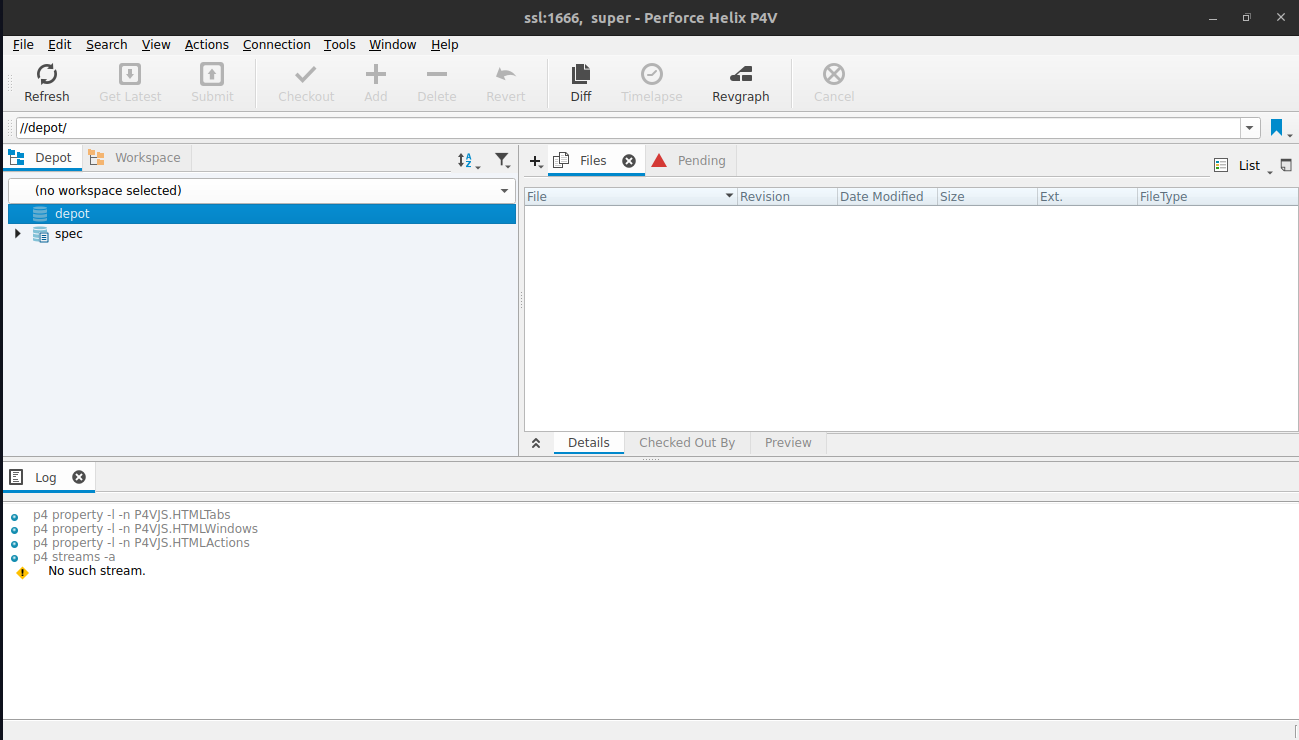
\includegraphics[width=\textwidth]{p4vlogin20231029.png}
      \caption{p4v login}
      \label{fig:p4v login}
\end{figure}

\subsection{Setup Godot}
Setting up Godot game engine is relatively easy compared to other game engines like Unity\textsuperscript{\texttrademark}
or Unreal Engine\textsuperscript{\texttrademark}. Godot is lightweight and there are basically two options to get hold
of the application:
\begin{itemize}
    \item Download pre-build application specific to host machine OS and programming language (GDScript or .Net)
    \href{https://godotengine.org/download/linux/}{\color{blue}Download page}
    \item Build from source following instructions 
    \href{https://docs.godotengine.org/en/stable/contributing/development/compiling/index.html}{\color{blue}Build from source}.
\end{itemize}
For the purpose of this paper the first approach was adopted by downloading the Godot 4.1.2 stable version for Linux.
After downloading and unpacking, Godot is ready to use:
\begin{figure}[H]
    \centering
    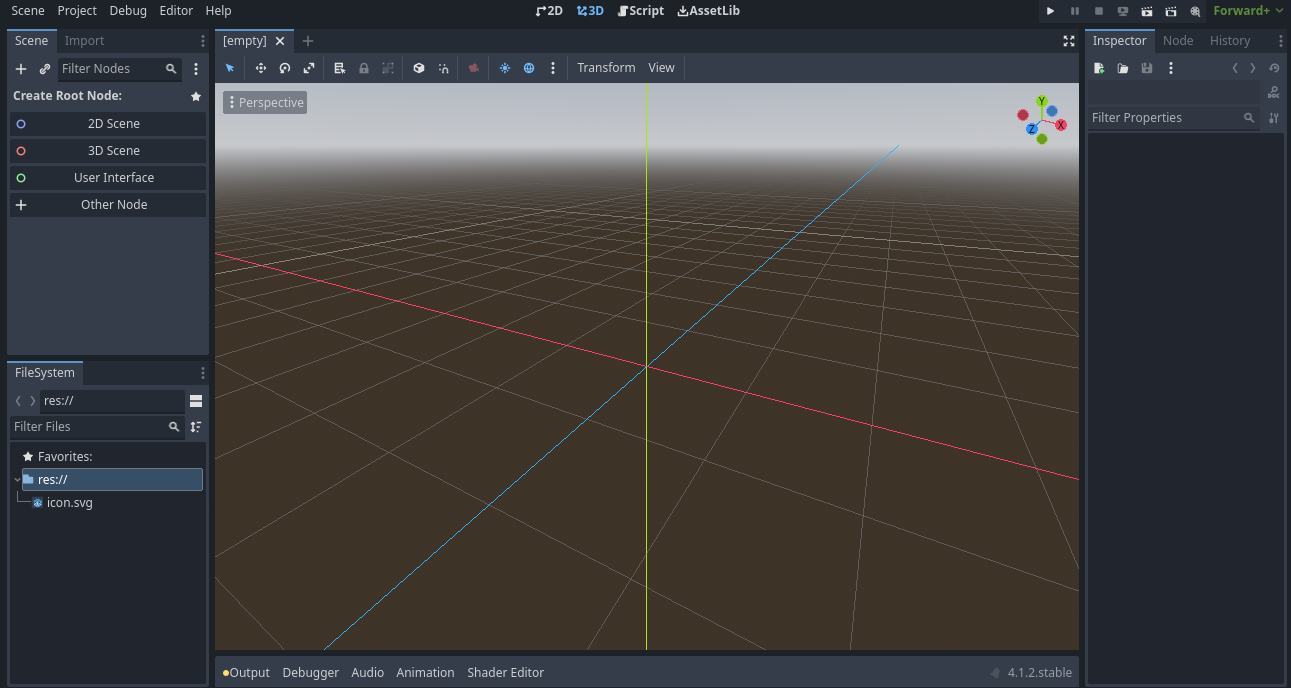
\includegraphics[width=\textwidth]{godotopen.png}
      \caption{godot editor}
      \label{fig:godot}
\end{figure}

\subsection{Development and version control}
%\begin{itemize}
%    \item 2D game using 
%    \href{https://docs.godotengine.org/en/stable/getting_started/first_2d_game/index.html}{\color{blue}Godot 2D game instructions}
%    \item create empty godot project
%    \item setup workspace for version control with perforce and initial commit
%    \item follow development steps with version control
%\end{itemize}
The final step before the start of the development is to prepare the server depot and local workspace areas, connect 
and initialize them by adding the first version of files from the Godot project. 
The following section details the development steps of a very simple 2D game based on instructions from the Godot 
tutorial at \href{https://docs.godotengine.org/en/stable/getting_started/first_2d_game/index.html}{\color{blue}Godot 2D game instructions}
using Perforce's Helix Core as version control system.
\begin{enumerate}
    \item First, start by setting up a new depot on the server. Login to perforce. Run from terminal:
        \begin{verbatim}
            $ p4 login
            $ p4v
        \end{verbatim}
    \item Choose Tools {$=>$} Administration (or press CTRL+SHIFT+A). This brings up Helix Admin.
    \item From Helix Admin, File {$=>$} New {$=>$} Depot. Enter a name for the depot (\textit{godot2d} in my case), 
    choose stream as depot type then press \colorbox{blue!30}{OK}. The new empty depot is created on the server. 
    Finally, close Helix Admin.
    \item Create TypeMap. TypeMap tells Perforce how to treate different type of files and what rules should be applied
    on the type of files when being edited. E.g. some binary files cannot be modified if someone else is also working 
    on it as conflicts cannot be resolved and in such cases either one or the other version of the file has to be retained 
    and the other will be dropped. For these files, it is better to use the \textit{+l} modifier which automatically
    locks the file so multiple users are not allowed to edit the file at the same time.
    \begin{verbatim}
        TypeMap:
            binary //....meta
            binary+wS //....exe
            +l //project_a/....obj
    \end{verbatim}
    The '...' symbol is a recursive wildcard in Perforce ('*' is non-recursive wildcard).
    In this example, all files ending with .meta should be treated as binary, the .exe files should be treated as binary
    with the 'w' and 'S' modifiers (always writable and using latest revision), whereas all .obj files in the project\_a
    folder should be locked. To create a TypeMap, open a terminal and type the following command:
    \begin{verbatim}
        $ p4 typemap
    \end{verbatim}
    The command brings up a typemap template that is already defined for several file types. Unfortunately,
    the default editor for p4v is not the most user-friendly, so it makes sense to switch the editor before calling the
    previous command. To switch the editor to nano, type:
    \begin{verbatim}
        $ p4 set P4EDITOR=nano
    \end{verbatim}
    Now, it is much easier to make changes to the template typemap.
    The following typemap will be used for the project at hand:
    \begin{verbatim}
        Typemap:
            binary+lS //....png
            text+lS //....import
            text+w //....gd
            text+w //....tscn
            binary //....godot
    \end{verbatim}
    \item Next up, a stream is to be created. Streams are useful assets in Perforce as they allow different
    teams to work on the project without distracting each other. E.g. 3D modellers can work on one stream and developers 
    on another one and once they are both happy with the outcome, the development stream can be merged to the 3D modellers'
    stream to make the changes available to them. In this example, only one stream will be created.
    To do this, click the Add tab button on the right pane and select Stream Graph. Then right click in any blank space
    and select New stream. Populate the input fields: \\
    Stream name: main \\
    Stream type: mainline \\
    Depot: godot2d \\
    Uncheck Create Workspace and Populate checkbox to avoid these automatic steps. These will be executed manually.
    \begin{figure}[H]
        \centering
        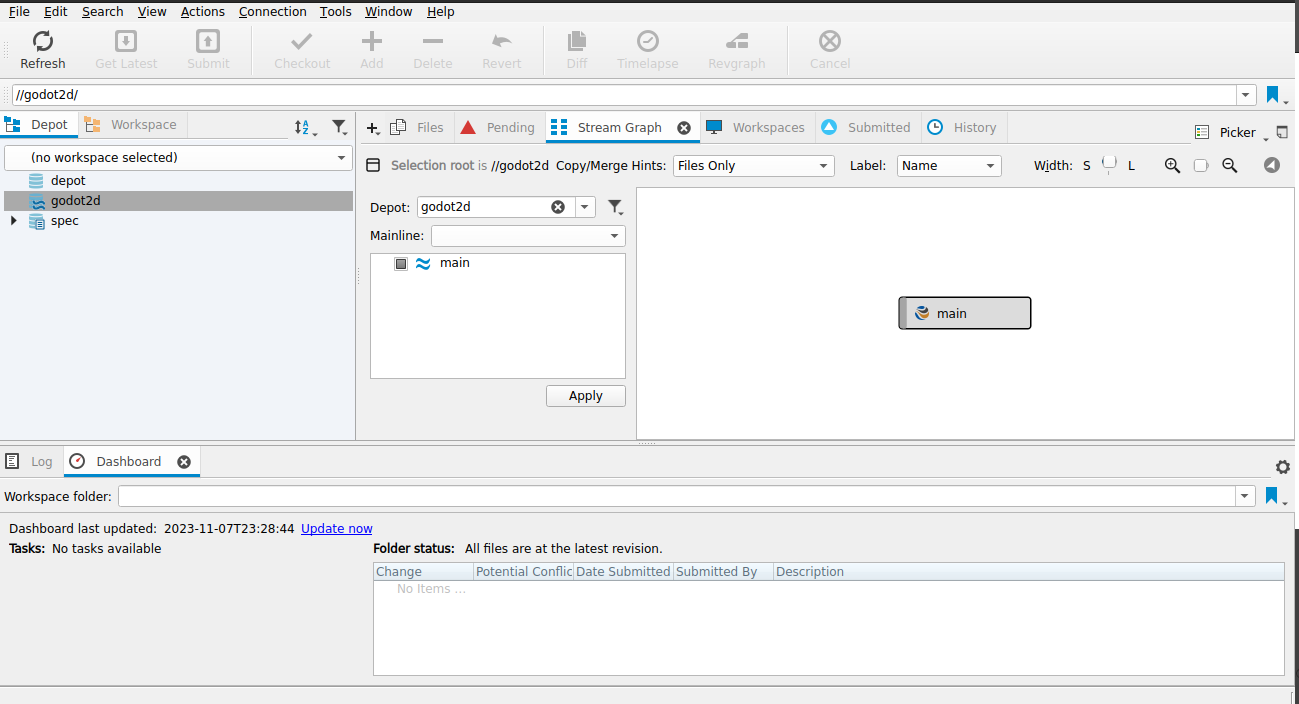
\includegraphics[width=\textwidth]{create-stream.png}
          \caption{new stream}
          \label{fig:new-stream}
    \end{figure}
    \item Next, a new workspace has to be created in p4v: click View {$=>$} Workspaces, right click on blank area on the
    right side when the Workspaces tab is active, click on new workspace. Instead of clicking, just press CTRL+N.
    \item Workspace name and root need to be given. The former usually follows the naming convention of 
    \textit{$<$user$>$\_$<$machine\_name$>$\_$<$project\_name$>$} which becomes in my case 
    \textit{super\_lefodor-HP\_godot2d}. The latter is set to any location on the local machine that ensures convenient
    working with the repository. Additionally, the stream is also to be filled out.
    \begin{figure}[H]
        \centering
        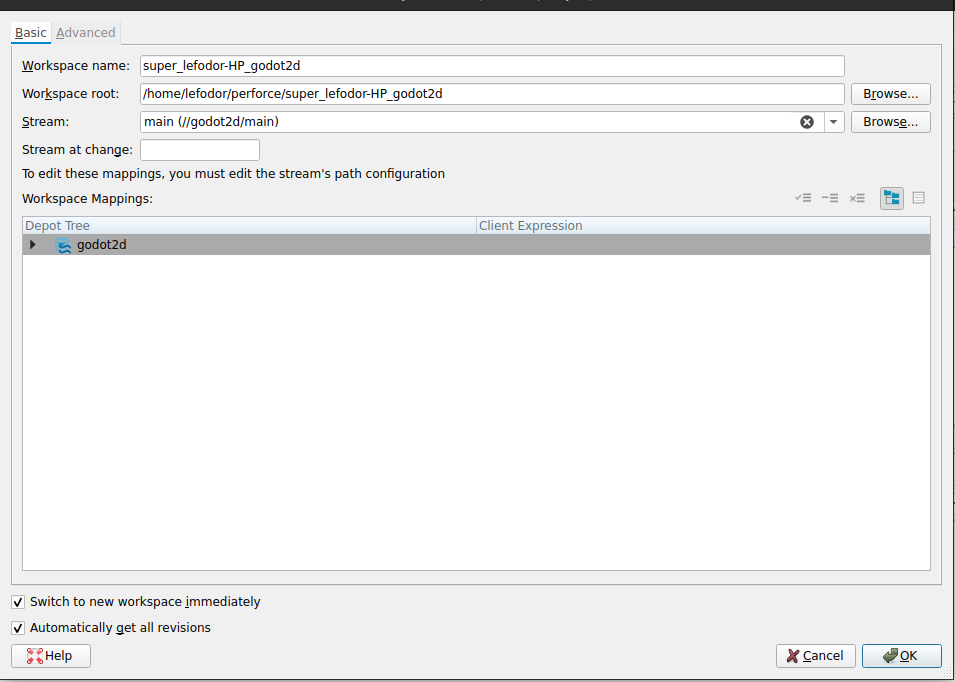
\includegraphics[width=\textwidth]{new-workspace2.png}
          \caption{new-workspace}
          \label{fig:new-workspace}
    \end{figure}
    Right click on all depots that are not required in the repository {$=>$} click Clear. After this step, only depot godot2d
    should have green pipe next to it. Then click on OK to create new workspace.
    \item Similarly to other version control systems, it is also possible to define a file that specifies files that are
    not subject to version control. In a new terminal window:
    \begin{verbatim}
        $ p4 set P4IGNORE=.p4ignore
        $ touch /home/lefodor/perforce/super_lefodor-HP_godot2d/.p4ignore
    \end{verbatim}
    In P4V, on the left pane right click on the file and click \textbf{Mark for Add} to add it to the default changelist, 
    and then hit \textbf{Submit} in the upper button bar while the file is selected.
    \item Add files to workspace. Copy blank Godot project folder to workspace root folder. Refresh P4V if needed to see
    the newly copied files in the left pane. Add the files to the default changelist and hit \textbf{Submit}. Only the 
    non-hidden files have been added to the workspace for version controll (note the small green icon next to files).
    \begin{figure}[H]
        \centering
        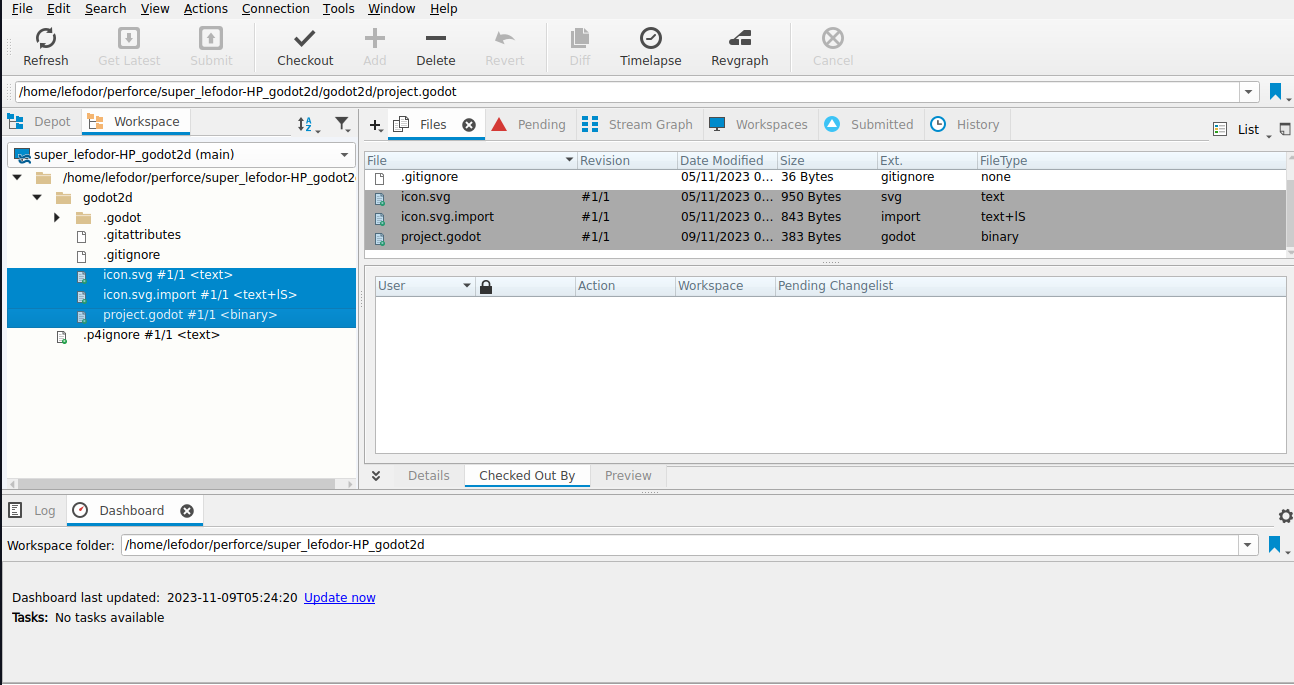
\includegraphics[width=\textwidth]{init-workspace.png}
          \caption{init-workspace}
          \label{fig:init-workspace}
    \end{figure}

    Having done the final step, the folder is ready to be shared and version controlled via the server depot and the 
    local workspace contents, currently 3 files are part of the repository of \textit{godot2d}.
\end{enumerate}
